%%%%%%%%%%%%%%%%%%%%%%%%%%%%%%%%%%%%%%%%%%%%%%%%%%%
%% LaTeX book template                           %%
%% Author:  Amber Jain (http://amberj.devio.us/) %%
%% License: ISC license                          %%
%%%%%%%%%%%%%%%%%%%%%%%%%%%%%%%%%%%%%%%%%%%%%%%%%%%

\documentclass[a4paper,spanish,11pt]{book}
\usepackage[T1]{fontenc}
\usepackage[utf8]{inputenc}
\usepackage{lmodern}
%%%%%%%%%%%%%%%%%%%%%%%%%%%%%%%%%%%%%%%%%%%%%%%%%%%%%%%%%
% Source: http://en.wikibooks.org/wiki/LaTeX/Hyperlinks %
%%%%%%%%%%%%%%%%%%%%%%%%%%%%%%%%%%%%%%%%%%%%%%%%%%%%%%%%%
\usepackage{hyperref}
\usepackage{graphicx}
\usepackage[spanish]{babel}

%\usepackage[english]{babel}
%\usepackage[utf8]{inputenc}

\usepackage{pgf,tikz}

\usetikzlibrary{shapes, calc, shapes, arrows, math, babel, positioning,lindenmayersystems}
\newcommand{\degre}{\ensuremath{^\circ}}
\usepackage{pgf,tikz,pgfplots}
\pgfplotsset{compat=1.15}
\usepackage{mathrsfs}
\usetikzlibrary{arrows}
%\pagestyle{empty}

\usepackage{amsmath,amssymb,textcomp}
\everymath{\displaystyle}

\usepackage{graphicx}
\usepackage{xcolor}

\usepackage{pdfpages}

\newcommand{\samedir}{\mathbin{\!/\mkern-5mu/\!}}

%%%%%%%%%%%%%%%%%%%%%%%%%%%%%%%%%%%%%%%%%%%%%%%%%%%%%%%%%%%%%%%%%%%%%%%%%%%%%%%%
% 'dedication' environment: To add a dedication paragraph at the start of book %
% Source: http://www.tug.org/pipermail/texhax/2010-June/015184.html            %
%%%%%%%%%%%%%%%%%%%%%%%%%%%%%%%%%%%%%%%%%%%%%%%%%%%%%%%%%%%%%%%%%%%%%%%%%%%%%%%%
\newenvironment{dedication}
{
   \cleardoublepage
   \thispagestyle{empty}
   \vspace*{\stretch{1}}
   \hfill\begin{minipage}[t]{0.66\textwidth}
   \raggedright
}
{
   \end{minipage}
   \vspace*{\stretch{3}}
   \clearpage
}

%%%%%%%%%%%%%%%%%%%%%%%%%%%%%%%%%%%%%%%%%%%%%%%%
% Chapter quote at the start of chapter        %
% Source: http://tex.stackexchange.com/a/53380 %
%%%%%%%%%%%%%%%%%%%%%%%%%%%%%%%%%%%%%%%%%%%%%%%%
\makeatletter
\renewcommand{\@chapapp}{}% Not necessary...
\newenvironment{chapquote}[2][2em]
  {\setlength{\@tempdima}{#1}%
   \def\chapquote@author{#2}%
   \parshape 1 \@tempdima \dimexpr\textwidth-2\@tempdima\relax%
   \itshape}
  {\par\normalfont\hfill--\ \chapquote@author\hspace*{\@tempdima}\par\bigskip}
\makeatother

%%%%%%%%%%%%%%%%%%%%%%%%%%%%%%%%%%%%%%%%%%%%%%%%%%%
% First page of book which contains 'stuff' like: %
%  - Book title, subtitle                         %
%  - Book author name                             %
%%%%%%%%%%%%%%%%%%%%%%%%%%%%%%%%%%%%%%%%%%%%%%%%%%%

% Book's title and subtitle
\title{\Huge \textbf{Preparación EVAU}  \\ \emph{}  \\\bigskip  \huge Matemáticas CCSS - 2º Bachillerato 
%\footnote{\url{}}
\\ \bigskip 
{
\foreach \k in {4}
{
  \tikz\draw[lindenmayer system={SierpArr,angle=60,axiom=X,step=200pt/2^\k,order=\k}]lindenmayer system;
}
}
} 
% Author
\author{\textsc{Departamento de Matemáticas}\thanks{\url{http://www.iespedrocerrada.org/}}}
\date{}

\pgfdeclarelindenmayersystem{SierpArr}{
  \symbol{X}{\pgflsystemdrawforward}
  \symbol{Y}{\pgflsystemdrawforward}
  \rule{X -> Y-X-Y}
  \rule{Y -> X+Y+X}
}

 

\begin{document}



%\frontmatter
\maketitle


%%%%%%%%%%%%%%%%%%%%%%%%%%%%%%%%%%%%%%%%%%%%%%%%%%%%%%%%%%%%%%%
% Add a dedication paragraph to dedicate your book to someone %
%%%%%%%%%%%%%%%%%%%%%%%%%%%%%%%%%%%%%%%%%%%%%%%%%%%%%%%%%%%%%%%
\begin{dedication}

\textbf{ATRIBUCIONES:} El material que aparece a continuación es autoría de \textbf{Julio García Galavis}. \\ Nuestro más sentido \textbf{agradecimiento} a su trabajo y que se encuentra en su página web\footnote{\url{http://matematicasentumundo.es/PAU/PAU.htm}}.


\bigskip 

\textbf{Licencia:} El contenido del documento se publica con licencia Attribution Share Alike (CC BY-SA)

\includegraphics[scale=0.2]{attribution-share-alike-creative-commons-license.png} 



\end{dedication}

%%%%%%%%%%%%%%%%%%%%%%%%%%%%%%%%%%%%%%%%%%%%%%%%%%%%%%%%%%%%%%%%%%%%%%%%
% Auto-generated table of contents, list of figures and list of tables %
%%%%%%%%%%%%%%%%%%%%%%%%%%%%%%%%%%%%%%%%%%%%%%%%%%%%%%%%%%%%%%%%%%%%%%%%
%\tableofcontents
%\listoffigures
%\listoftables

%\mainmatter

\chapter{Álgebra}

A continuación aparecen los ejercicios de la EVAU del bloque de álgebra de los últimos seis años con las soluciones. Se recomienda trabajarlos para preparar la EVAU. En caso de necesitar consultar el desarrollo de la solución paso a paso se deberá consultar el documento específico de la prueba y año que aparece en la siguiente web\footnote{\url{http://matematicasentumundo.es/PAU/PAU.htm}}:\\

\begin{center}

\includegraphics[scale=0.6]{qr_ejercicios_evau.png} 

\end{center}


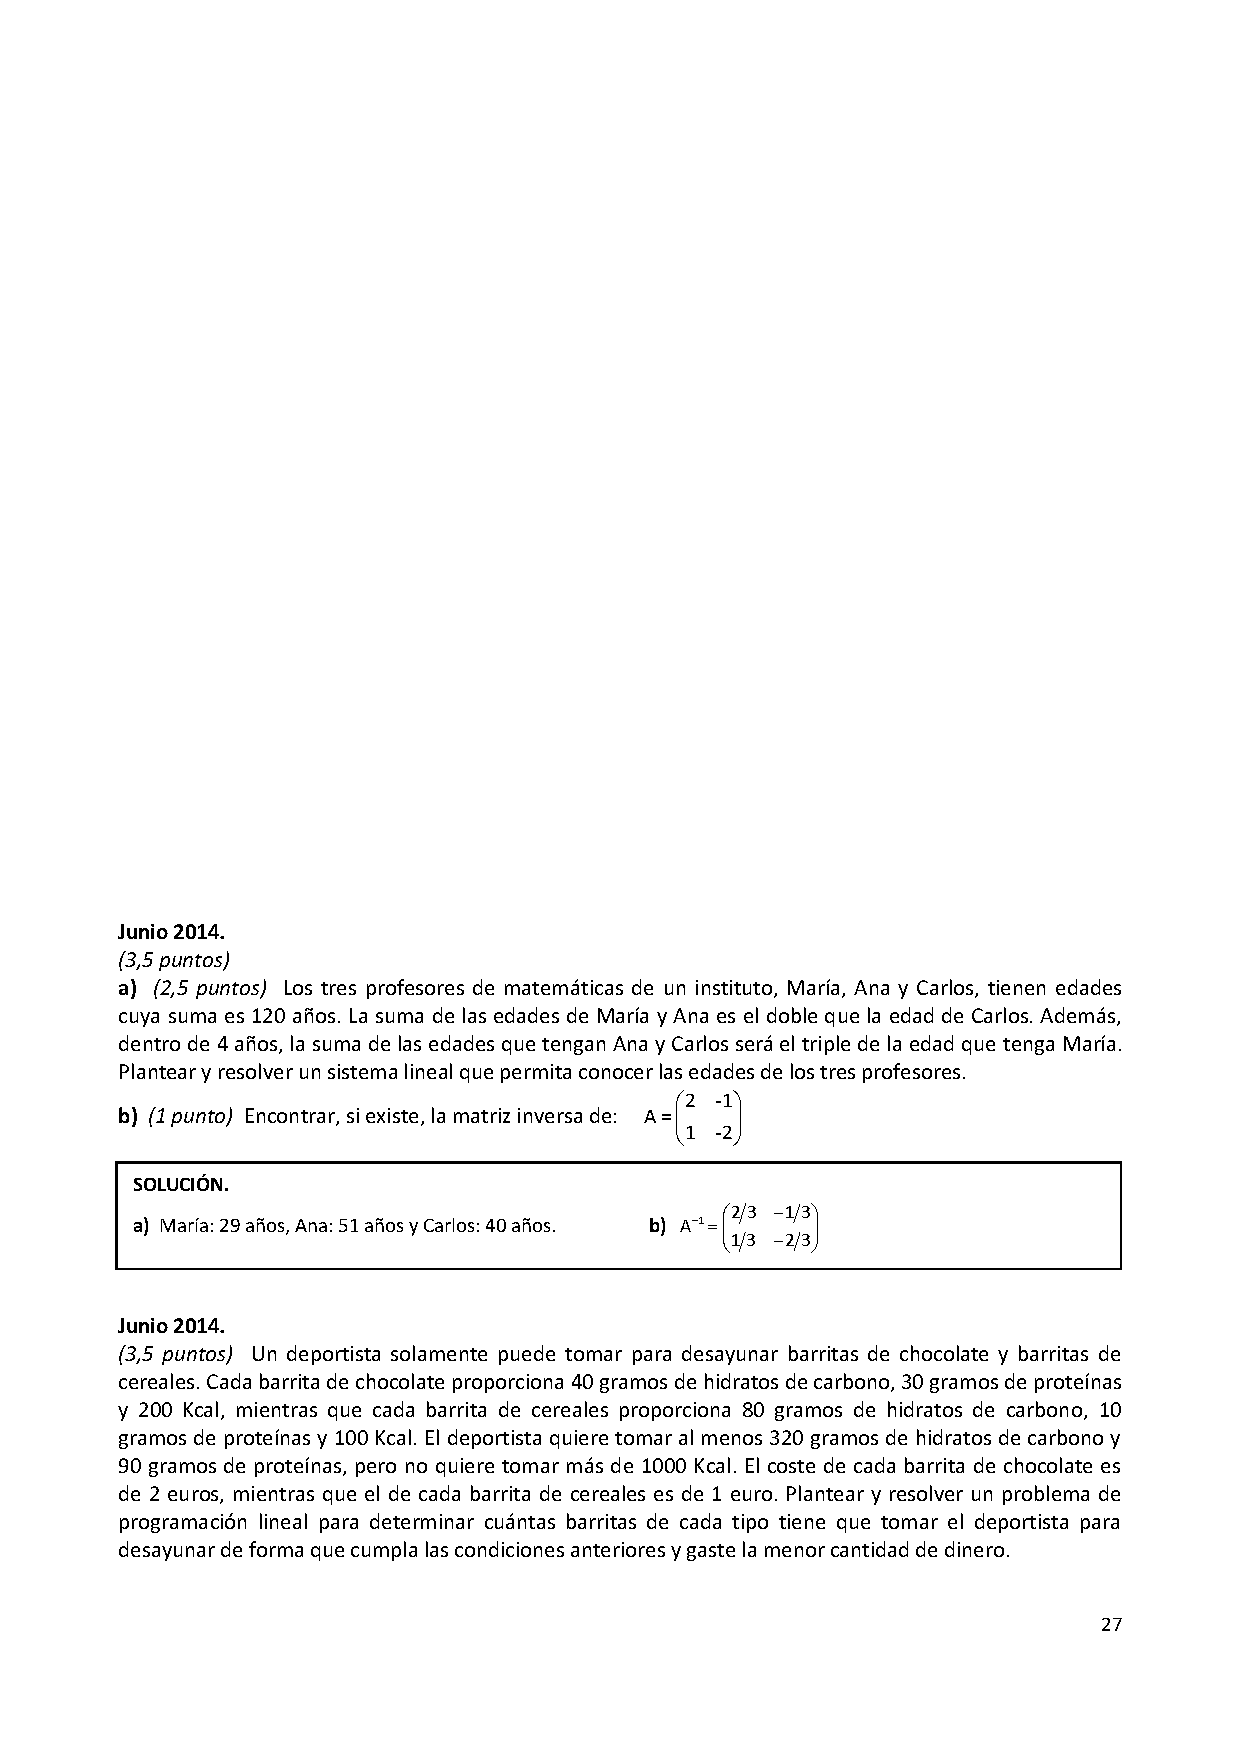
\includepdf[pages=-, scale=0.9]{prepevaualgebra.pdf}



\chapter{Análisis}

A continuación aparecen los ejercicios de la EVAU del bloque de análisis de los últimos seis años con las soluciones. Se recomienda trabajarlos para preparar la EVAU. En caso de necesitar consultar el desarrollo de la solución paso a paso se deberá consultar el documento específico de la prueba y año que aparece en la siguiente web\footnote{\url{http://matematicasentumundo.es/PAU/PAU.htm}}:\\

\begin{center}

\includegraphics[scale=0.6]{qr_ejercicios_evau.png} 

\end{center}


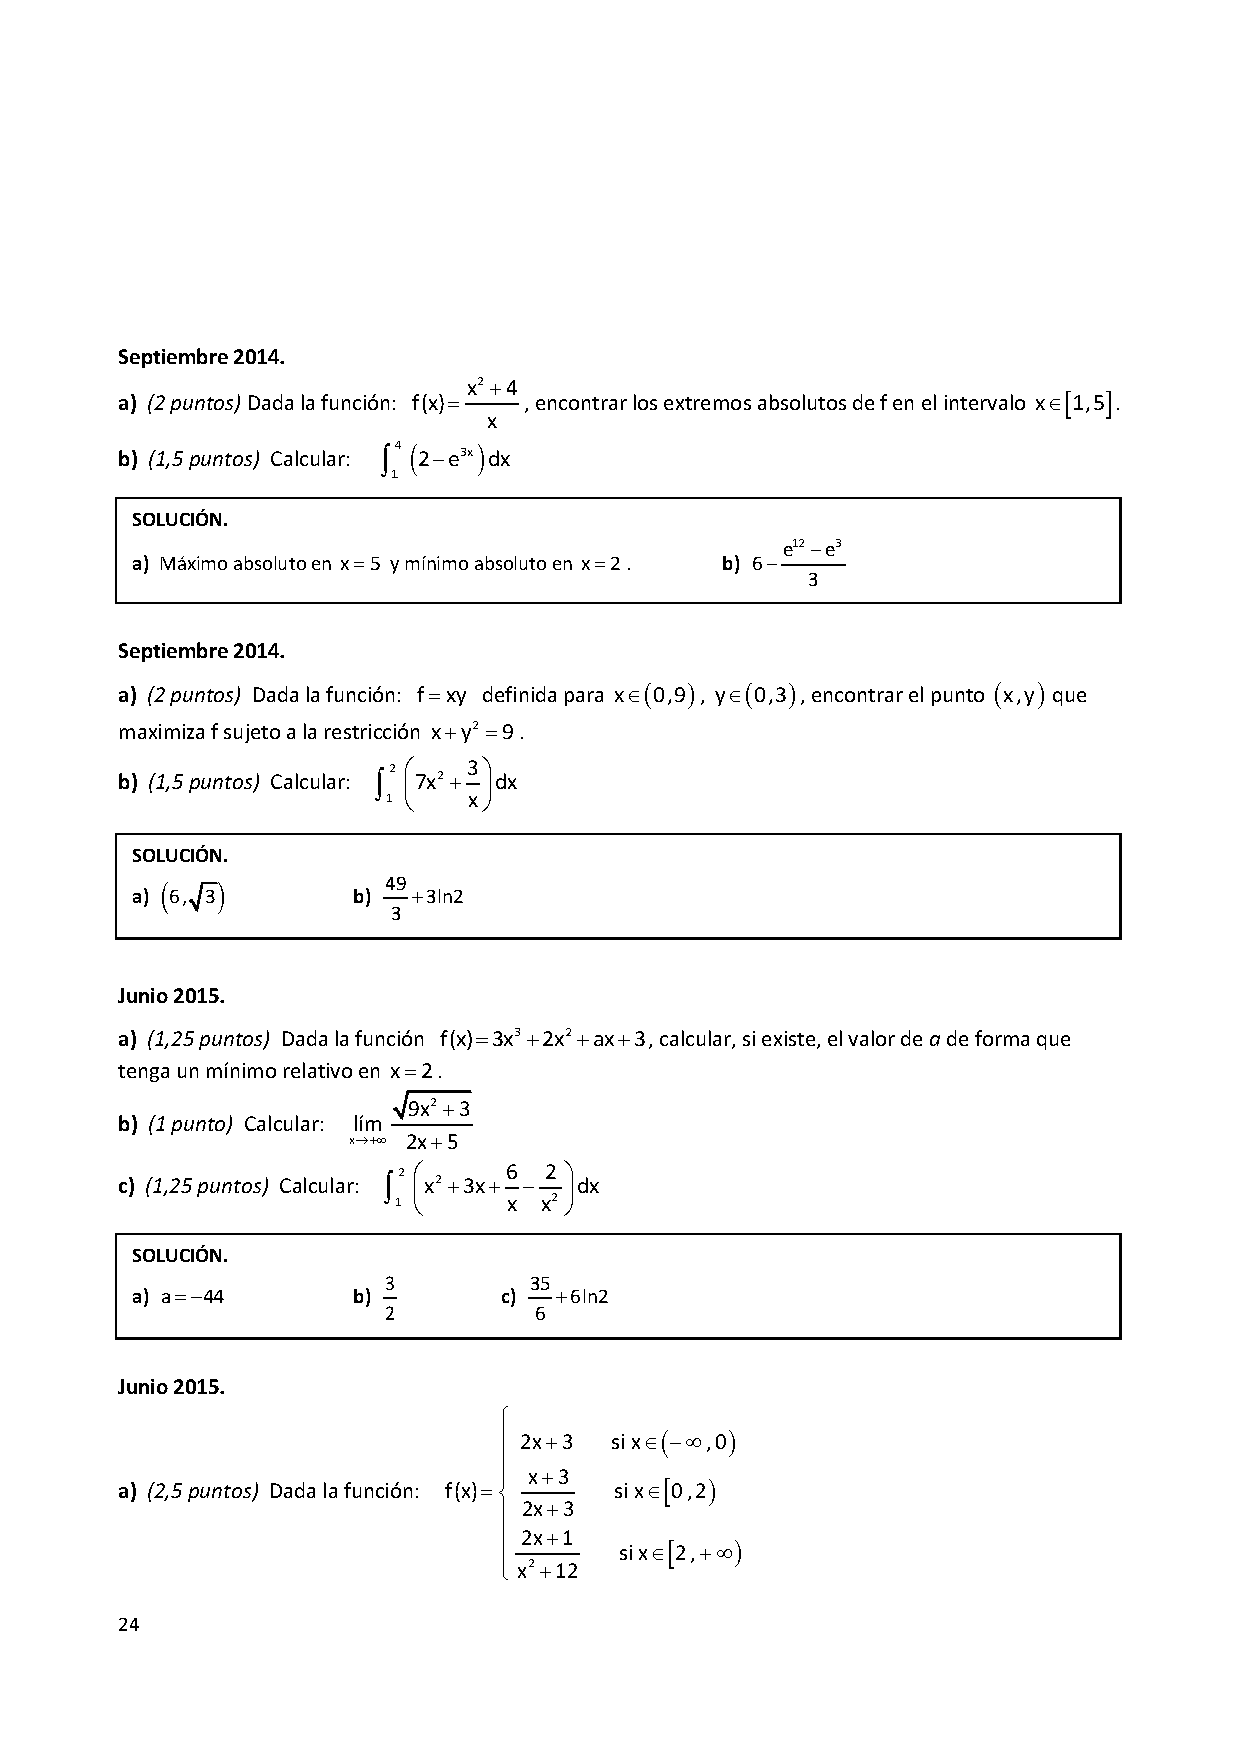
\includepdf[pages=-, scale=0.9]{prepevauanalisis.pdf}

\chapter{Probabilidad y Estadística}

A continuación aparecen los ejercicios de la EVAU del bloque de probabilidad y estadística de los últimos seis años con las soluciones. Se recomienda trabajarlos para preparar la EVAU. En caso de necesitar consultar el desarrollo de la solución paso a paso se deberá consultar el documento específico de la prueba y año que aparece en la siguiente web\footnote{\url{http://matematicasentumundo.es/PAU/PAU.htm}}:\\

\begin{center}

\includegraphics[scale=0.6]{qr_ejercicios_evau.png} 

\end{center}


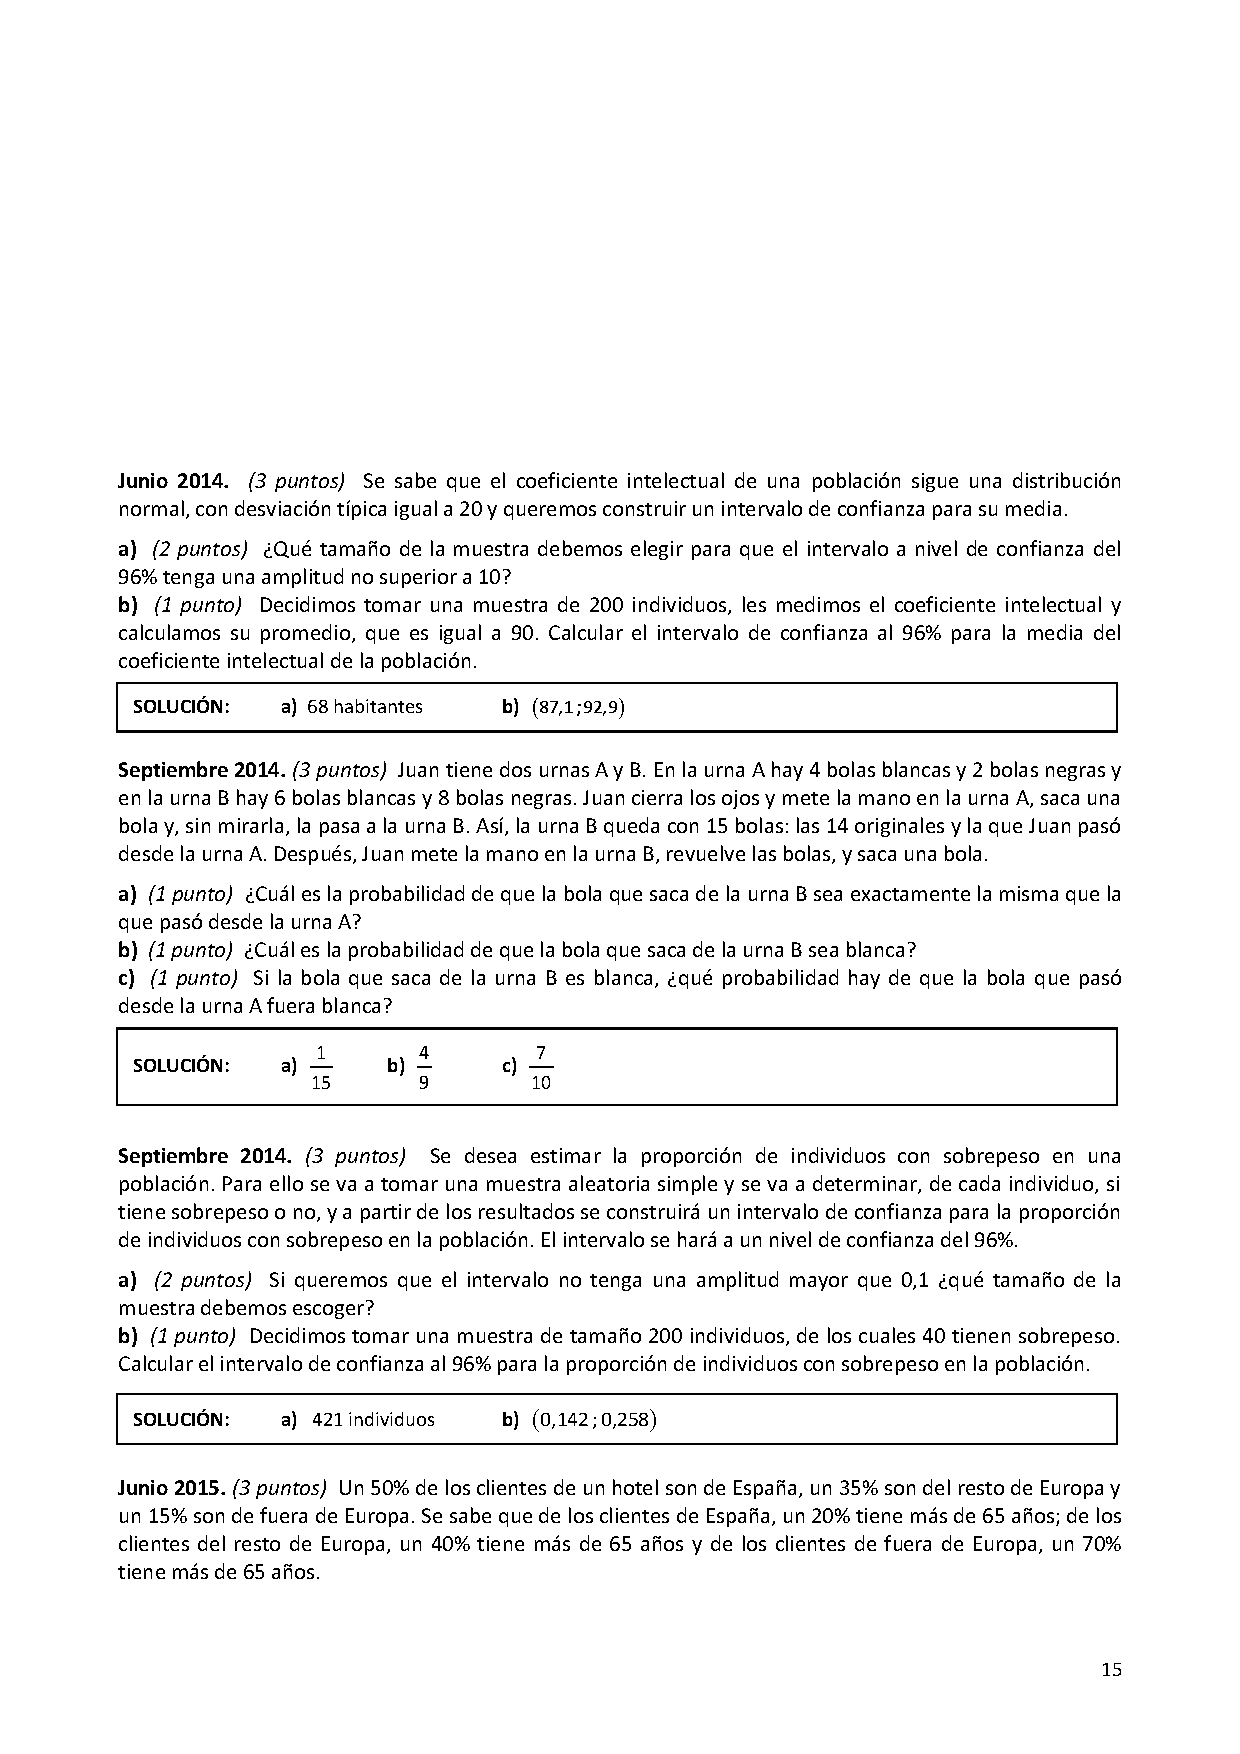
\includepdf[pages=-, scale=0.9]{prepevauprobabilidad.pdf}










\end{document}